\newcommand{\DoNotLoadEpstopdf}{}
\documentclass[11pt]{article}
\usepackage[T1]{fontenc}
\usepackage{lmodern}
\usepackage[margin=1in]{geometry}
\usepackage{amsmath,amssymb,amsthm,mathtools}
\usepackage{microtype,enumitem,needspace,placeins,xcolor,tikz,booktabs}
\usetikzlibrary{arrows.meta,positioning,calc}
\usepackage[colorlinks=true,linkcolor=blue!45!black,citecolor=blue!45!black,urlcolor=blue!45!black]{hyperref}
\hypersetup{pdftitle={A Nearly Quartic Separation Between Randomized and Quantum Query Complexity},pdfauthor={OpenAI}}
\newtheorem{theorem}{Theorem}[section]
\newtheorem{proposition}[theorem]{Proposition}
\newtheorem{lemma}[theorem]{Lemma}
\newtheorem{corollary}[theorem]{Corollary}
\theoremstyle{definition}
\newtheorem{definition}[theorem]{Definition}
\newtheorem{remark}[theorem]{Remark}
\newcommand{\R}{\mathrm R}
\newcommand{\Q}{\mathrm Q}
\newcommand{\D}{\mathrm D}
\newcommand{\E}{\mathbb E}
\newcommand{\bits}{\{0,1\}}
\newcommand{\bs}{\operatorname{bs}}
\newcommand{\poly}{\operatorname{poly}}
\DeclarePairedDelimiter{\norm}{\lVert}{\rVert}
\DeclarePairedDelimiter{\abs}{\lvert}{\rvert}
\DeclarePairedDelimiter{\ip}{\langle}{\rangle}
\setlist[enumerate]{label=\textup{(\roman*)},leftmargin=*}
\setlength{\emergencystretch}{1.5em}
\allowdisplaybreaks[1]

\title{A Nearly Quartic Separation Between\texorpdfstring{\\}{ }Randomized and Quantum Query Complexity}
\author{OpenAI}
\date{October 5, 2026}
\begin{document}
\maketitle
\begin{abstract}
We construct total Boolean functions with a nearly quartic separation
between bounded-error randomized and quantum query complexity.
Writing these complexities as $\R(f)$ and $\Q(f)$, the examples rule
out every universal bound $\R(f)=O((1+\Q(f))^\alpha)$ with
$\alpha<4$. Thus the known quartic upper bound has the optimal
exponent, disproving the conjectured cubic bound. Both complexities
count worst-case bit queries with error at most $1/3$ on every input.
\end{abstract}
\section{Introduction}\label{sec:introduction}

How much can a quantum algorithm reduce the number of input bits needed
to compute a total Boolean function? Let $f:\bits^n\to\bits$. We write
$\R(f)$ and $\Q(f)$ for the minimum worst-case numbers of bit queries made
by randomized and quantum algorithms that compute $f$ with error at most
$1/3$ on every input. Quantum queries use the standard oracle
\[
 O_x\lvert i,b,z\rangle=\lvert i,b\oplus x_i,z\rangle.
\]
Computation between queries is unrestricted. In particular, all query
bounds in this paper are worst-case bounds, including over internal
randomness and measurement outcomes.

Polynomial relations between these two measures express a basic
restriction on quantum speedups for total functions. To ask for the sharp
power without imposing a particular logarithmic correction, define
\begin{equation}\label{eq:alpha}
 \alpha_{\mathrm{tot}}=
 \inf\left\{\alpha\ge0:
 \begin{array}{l}
 \text{there exists }C_\alpha<\infty\text{ such that, for every }n\ge1\nobreak\text{ and}\smallskip\\
 f:\bits^n\to\bits,\quad
 \R(f)\le C_\alpha(1+\Q(f))^\alpha
 \end{array}\right\}.
\end{equation}
The additive $1$ includes constant functions. We prove the following.

\begin{theorem}\label{thm:main}
The optimal power is $\alpha_{\mathrm{tot}}=4$.
More precisely, $\R(f)=O((1+\Q(f))^4)$ for every total Boolean function.
For each fixed integer $k\ge2$, there are positive constants $c_k,C_k,b_k$
and total Boolean functions $F_{k,m}$, for all sufficiently large powers
of four $m$, such that
\begin{equation}\label{eq:main-family}
 \Q(F_{k,m})\le C_k\sqrt m\,(\log m)^{b_k},
 \qquad
 \R(F_{k,m})\ge c_k\frac{m^{2-1/k}}{(\log m)^2}.
\end{equation}
\end{theorem}

The universal upper bound is known. The contribution is the family in
\eqref{eq:main-family}, which rules out every smaller power, including
the conjectured cubic relation.

\subsection{Historical context}

Grover's search algorithm~\cite{Grover96} gives the basic quadratic
speedup for the OR function, with a matching quantum lower bound
\cite{BBBV97}. Beals, Buhrman, Cleve, Mosca, and de Wolf~\cite{BBCMW01}
proved the general polynomial relation $\D(f)=O(\Q(f)^6)$, where
$\D(f)$ is exact deterministic query complexity. Their result builds
on the combinatorial and polynomial measures studied by
Nisan~\cite{Nisan91} and Nisan and Szegedy~\cite{NisanSzegedy94}.
Thus totality rules out the exponential query speedups possible for
partial functions, but it leaves a substantial range of possible powers.

Pointer constructions introduced by G\"o\"os, Pitassi, and
Watson~\cite{GPW15} and developed by Ambainis, Balodis, Belovs, Lee,
Santha, and Smotrovs~\cite{ABBLSS17} gave a nearly quartic separation
between deterministic and quantum queries. For bounded-error randomized
queries, Aaronson, Ben-David, and Kothari~\cite{ABK16} introduced the
cheat-sheet framework and obtained a power-$5/2$ separation, up to
logarithmic factors. This framework places certificates in an array
whose correct address is determined by answers to partial-function
instances. Improvements in those partial-function separations led to
power $8/3-o(1)$ by Tal~\cite{Tal20}, and then $3-o(1)$ by Bansal
and Sinha~\cite{BS21} and independently Sherstov, Storozhenko, and
Wu~\cite{SSW23}.

On the upper-bound side, Aaronson, Ben-David, Kothari, Rao, and
Tal~\cite{ABKRT21}, using Huang's sensitivity theorem~\cite{Huang19},
proved $\D(f)=O(\Q(f)^4)$. They conjectured that randomized complexity
satisfies the stronger relation $\R(f)=O(\Q(f)^3)$
\cite[Conjecture~2]{ABKRT21}. Theorem~\ref{thm:main} disproves that
conjecture and shows that the quartic upper bound already has the
optimal power for bounded-error randomized complexity.

There is also a direct connection to algorithms that compare candidate
witnesses. Quantum minimum finding~\cite{DurrHoyer96}, sink finding
\cite{SYZ04}, and king finding in tournaments~\cite{MPS23} provide
related search procedures. Recent constructions of Ben-David and
Kothari~\cite{BK26} and Ambainis, Iraids, and Kokainis~\cite{AIK26}
use comparisons of candidate witnesses to separate certificate
complexity from randomized and quantum query complexity. Certificate
complexity measures the worst-case size of a smallest partial input
assignment that fixes the function value. Their nearly quartic
separations between certificate and quantum complexity concern a
different classical measure, but their comparison-based viewpoint is
particularly relevant here.

\subsection{The construction and its two analyses}

The input is organized into $m$ columns. Each column $i$ contains a string
$X_i$ of $m$ bits and an array of certificate cells. The address of the
relevant cell is the vector of answers to several disjoint instances
of a partial function. Quantumly these answers are cheap to obtain on
promised inputs; classically they are hard to guess. Each cell stores
pointers to positions in all the other strings $X_j$, together with a
circuit transcript certifying the address.

A column wins when its own string is all ones, its address is defined,
and its certificate is correct and points to a zero in every other
column. The total function asks whether a winner exists. There can be
at most one. An incorrect address or transcript simply fails verification;
the input to the total function carries no promise.

The direction of the pointers matters. A true winner can use its own
certificate to disqualify every opponent. Conversely, no cell in any
opponent can point to a zero in the winner's all-one string. Thus a cheap
quantum comparison favors the winner with high probability even if the
opponent's address instances violate their promises. Comparisons between
two non-winners may have arbitrary probabilities. Section~\ref{sec:quantum}
proves a tournament lemma that permits precisely this behavior. It
produces a short list containing the winner in $\sqrt m$ times a
polylogarithmic number of queries, after which quantum search checks the
certificates.

The classical proof starts with one independently hidden zero in every
$X_i$ and blank certificate cells. We choose a uniformly random column,
erase its zero, and fill its correctly addressed cell. These two changes
produce a winner. A randomized algorithm can distinguish the two inputs
only by finding the erased zero or querying the filled cell. The first
event is unlikely for a uniformly chosen column; the second requires
either many address queries in that column or a correct guess of an
entire vector of hard answers. An adaptive direct-product argument makes
this last assertion precise without conditioning on the algorithm's
choice of which columns to investigate.

The tournament analysis is useful independently of this construction.
It uses the actual probabilities of comparisons as multiplicative
weights; fresh coherent workspaces and amplitude amplification sample
those weights exactly. Only comparisons involving a genuine winner
need to be reliable. This extends the candidate-comparison approach
to the arbitrary behavior caused here by off-promise address inputs.
The classical analysis combines the planted input with a standard
per-instance-capped direct-product argument
\cite{Shaltiel03,Drucker12}; the separate cell arrays let this argument
charge the cost of addressing many possible winners.

Section~\ref{sec:construction} defines the function and its certificates.
Sections~\ref{sec:quantum} and~\ref{sec:classical} prove the two bounds in
\eqref{eq:main-family}; Section~\ref{sec:exponent} derives the optimal
power. Appendix~\ref{sec:upper} gives a self-contained proof of the known
quartic upper bound. The only external lower-bound input is the
Forrelation theorem stated in Section~\ref{sec:construction}.

\subsection{Conventions}

We write $[m]=\{1,\ldots,m\}$ and use logarithms to base two, except in
expressions where changing the base only changes an absolute constant.
Constants in bounds for $F_{k,m}$ may depend on the fixed integer $k$.
A partial Boolean function is specified on a subset of $\bits^N$;
its algorithms must be correct on that subset. The quantum routines used
here have a fixed query cap on every input, including inputs outside the
promise. A circuit transcript lists proposed values of the non-input
gates; the actual input bits are read directly when a gate check needs them.

\section{An addressed certificate with outward pointers}
\label{sec:construction}

We construct a total function whose accepting certificate belongs to one
column.  The certificate must certify the answers to several Forrelation
instances and point to a zero in every other column.  The latter requirement
will let a genuine accepting column defeat any competitor, even when that
competitor's Forrelation instances violate their promise.

Throughout the construction, fix an integer $k\geq 2$ and let $m$ tend to
infinity through powers of four.  Constants in $O_k(\cdot)$ may depend on
$k$, which remains fixed as $m$ grows.  Write $[m]=\{1,\ldots,m\}$.

\subsection{The partial function and its exact circuit}

We use the $k$-fold Forrelation problem introduced by Aaronson and
Ambainis~\cite{AA18}, with the thresholds analyzed by Bansal and
Sinha~\cite{BS21}. Let $H$ be the normalized Walsh--Hadamard matrix of order $m$, and let
$u=m^{-1/2}(1,\ldots,1)^{\mathsf T}$.  We identify a bit $a$ with the sign
$(-1)^a$.  For a sign vector $z$, write $D_z$ for the diagonal matrix with
diagonal $z$.  Given $k$ sign vectors $z_1,\ldots,z_k\in\{\pm1\}^m$, put
\begin{equation}\label{eq:forrelation-form}
 \Phi(z_1,\ldots,z_k)
 =u^{\mathsf T}D_{z_1}H D_{z_2}H\cdots H D_{z_k}u,
 \qquad \delta=2^{-5k}.
\end{equation}
Define the partial Boolean function $P=P_{k,m}$ on $km$ bits by
\begin{equation}\label{eq:forrelation-promise}
 P(z_1,\ldots,z_k)=
 \begin{cases}
  1,&\Phi(z_1,\ldots,z_k)\geq\delta,\\
  0,&|\Phi(z_1,\ldots,z_k)|\leq\delta/2,
 \end{cases}
\end{equation}
and leave it undefined on all other inputs.  The two displayed cases are
disjoint.  Query complexity for this partial function requires correctness
only on its domain.

\begin{lemma}\label{lem:forrelation}
For each fixed integer $k\geq2$, the functions $P_{k,m}$ have the following
properties.
\begin{enumerate}
 \item For all sufficiently large powers of four $m$,
 \begin{equation}\label{eq:L-def}
  \R(P_{k,m})>L,
  \qquad
  L=\left\lfloor
       \frac{m^{1-1/k}}{(\log_2 m)^2}
     \right\rfloor.
 \end{equation}
 \item For every $0<\eta<1/2$, a quantum algorithm uses
 $O_k(1+\log(1/\eta))$ bit queries and returns $P_{k,m}$ with error at most
 $\eta$ on every input in its domain.  The algorithm can be implemented
 coherently, retaining its workspace.  On every input, promised or not, it
 produces a bit when its output register is measured.
 \item There is a Boolean circuit $C=C_{k,m}$ of fan-in at most two and
 size $S=S_{k,m}=O_k(m(\log m)^2)$ with two output bits $d,b$ such that
 \[
  d=1\quad\Longleftrightarrow\quad P_{k,m}\text{ is defined},
  \qquad d=1\quad\Longrightarrow\quad b=P_{k,m}.
 \]
 The circuit computes these outputs exactly on every input.
\end{enumerate}
\end{lemma}

\begin{proof}
Theorem~1.3 and Corollary~1.4 of Bansal and Sinha~\cite{BS21} apply to
exactly the normalized form and thresholds in
\eqref{eq:forrelation-form}--\eqref{eq:forrelation-promise}.  They give,
for fixed $k$ and error $1/3$,
\[
 \R(P_{k,m})=
 \Omega_k\!\left(
   \left(\frac{m}{\log(km)}\right)^{1-1/k}
 \right).
\]
This exceeds the value of $L$ in \eqref{eq:L-def} for all sufficiently
large $m$.

For the quantum algorithm, prepare $u$, apply the unitary product in
\eqref{eq:forrelation-form}, in its right-to-left order, and test the
projection onto $u$.  Each $D_{z_h}$ uses one phase query, implemented by
the standard bit oracle, while $H$ and the projection require no queries.
The projection succeeds with probability $\Phi^2$.  This probability is
at least $\delta^2$ on a 1-input and at most $\delta^2/4$ on a 0-input.
Independent repetitions and a threshold between these two numbers give
error $\eta$ with $O_k(1+\log(1/\eta))$ repetitions.  The measurement
outcomes and the final threshold decision can instead be computed into
registers and retained, giving the claimed coherent implementation.

For the circuit, let $W=\sqrt m\,H$, whose entries are $\pm1$.  The scalar
\[
 N=z_1^{\mathsf T}W D_{z_2}W\cdots W D_{z_k}(1,\ldots,1)^{\mathsf T}
\]
is an integer, and
\[
 \Phi=\frac{N}{M_{k,m}},
 \qquad M_{k,m}=m(\sqrt m)^{k-1}.
\]
The denominator is an integer because $m$ is a power of four.  Compute
$N$ by $k-1$ unnormalized Walsh--Hadamard transforms, coordinatewise sign
changes, and a final signed sum.  Each transform uses $O(m\log m)$
additions and subtractions by the usual butterfly recursion.  All
intermediate integers have absolute value at most $m^{O(k)}$, so
$O_k(\log m)$ bits suffice.  Binary additions, subtractions, sign changes,
and comparisons have fan-in-two Boolean circuits of size linear in this
bit length.  Consequently the entire arithmetic circuit has Boolean size
$O_k(m(\log m)^2)$.

Finally, the two tests in \eqref{eq:forrelation-promise} are the exact
integer comparisons
\[
 2^{5k}N\geq M_{k,m},
 \qquad 2^{5k+1}|N|\leq M_{k,m}.
\]
Set $d$ to the disjunction of these comparisons and $b$ to the first
comparison.  This adds only $O_k(\log m)$ gates and proves the last
assertion.
\end{proof}

The exact circuit serves a different purpose from the quantum algorithm.
The algorithm will propose an address.  A transcript of the circuit will
certify that this address consists of defined, correct answers, including
on inputs where an arbitrary proposed address has no reason to be correct.

\subsection{The total function}

Set
\begin{equation}\label{eq:r-def}
 r=\lceil20\log_2m\rceil,
 \qquad \ell=\log_2m.
\end{equation}
The input has $m$ columns.  Column $i\in[m]$ contains the following bits:
\begin{enumerate}
 \item A string $X_i\in\bits^m$.
 \item Strings $A_{i,1},\ldots,A_{i,r}\in\bits^{km}$, with no promise
 imposed on them.
 \item A cell $B_{i,s}$ for each address $s\in\bits^r$.  This cell
 contains a pointer $p_{i,s,j}\in[m]$ for each $j\ne i$, encoded by
 $\ell$ bits using a fixed bijection, and an alleged evaluation transcript
 of $C_{k,m}$ on each $A_{i,h}$, $h\in[r]$.
\end{enumerate}
An evaluation transcript consists of one bit for every non-input gate of
$C_{k,m}$, including its output gates.  Circuit inputs are the actual bits
of $A_{i,h}$; they need not be copied into the transcript.  We count these
non-input gates in $S$.

Call column $i$ a \emph{winner} if $X_i=1^m$, every $P(A_{i,h})$ is
defined, and the cell at its true address
\begin{equation}\label{eq:true-address}
 s_i=(P(A_{i,1}),\ldots,P(A_{i,r}))
\end{equation}
contains correct evaluation transcripts and pointers satisfying
\begin{equation}\label{eq:outward-pointers}
 X_j[p_{i,s_i,j}]=0\qquad\text{for every }j\ne i.
\end{equation}
Define $F_{k,m}$ to be 1 if a winner exists, and 0 otherwise.  This is a
total Boolean function: all the preceding conditions are predicates on
the input bits, and no promise is made about the $A$-strings, the pointers,
or the transcripts.

The addressed transcripts have the certificate role used in cheat-sheet
constructions~\cite{ABK16}, while pointers between columns also occur in
earlier query-complexity separations~\cite{GPW15,ABBLSS17}. Here the pointers have
a specific outward orientation: an accepting column supplies a direct
zero witness against every competitor.  In particular, there can be at
most one winner, since a winner's pointer to another column certifies that
the latter is not all ones.  Figure~\ref{fig:outward} depicts this
condition.

\begin{figure}[t]
\centering
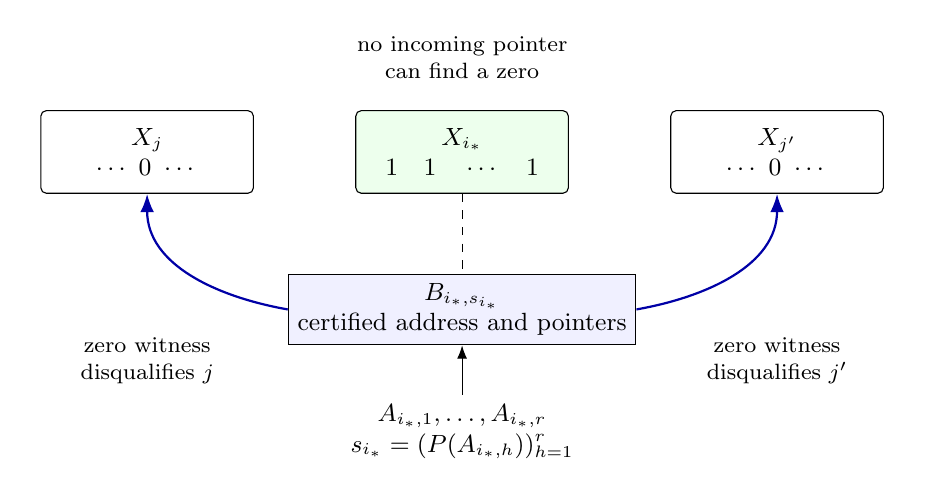
\begin{tikzpicture}[>=Latex,font=\small,
 col/.style={draw,rounded corners=2pt,minimum width=2.7cm,minimum height=1.05cm,align=center},
 cell/.style={draw,fill=blue!6,minimum width=3.7cm,minimum height=0.85cm,align=center}]
\node[col] (left) at (-4,1.8) {$X_j$\\$\cdots\ 0\ \cdots$};
\node[col,fill=green!7] (win) at (0,1.8) {$X_{i_\ast}$\\$1\quad1\quad\cdots\quad1$};
\node[col] (right) at (4,1.8) {$X_{j'}$\\$\cdots\ 0\ \cdots$};
\node[align=center,text width=3.7cm,font=\footnotesize] at (0,3.0) {no incoming pointer can find a zero};
\node[cell] (cert) at (0,-0.2) {$B_{i_\ast,s_{i_\ast}}$\\certified address and pointers};
\node[align=center] (addr) at (0,-1.75) {$A_{i_\ast,1},\ldots,A_{i_\ast,r}$\\$s_{i_\ast}=(P(A_{i_\ast,h}))_{h=1}^r$};
\draw[->] (addr) -- (cert);
\draw[->,thick,blue!65!black] (cert.west) to[out=170,in=-90] (left.south);
\draw[->,thick,blue!65!black] (cert.east) to[out=10,in=-90] (right.south);
\draw[dashed] (win.south) -- (cert.north);
\node[align=center,text width=2.8cm,font=\footnotesize] at (-4,-0.85) {zero witness\\disqualifies $j$};
\node[align=center,text width=2.8cm,font=\footnotesize] at (4,-0.85) {zero witness\\disqualifies $j'$};
\end{tikzpicture}
\caption{The relevant cell of a winning column points outward to a zero
in every other column; two such pointers are shown. Only the indicated
zeros are prescribed in the other columns. The cell's address is
computed from the partial-function answers and certified by stored
circuit transcripts. The winner's all-one string prevents every opponent
from disqualifying it, even at an incorrectly decoded address.}
\label{fig:outward}
\end{figure}

\FloatBarrier

We next make certificate verification precise.  For a specified pair
$(i,s)$, say that $i$ wins \emph{at address $s$} if $i$ is a winner and
$s=s_i$.

\Needspace{9\baselineskip}
\begin{lemma}\label{lem:local-tests}
For every input to $F_{k,m}$ and every pair $(i,s)\in[m]\times\bits^r$,
the assertion that $i$ wins at address $s$ is a conjunction of
\[
 K_{k,m}=m+(m-1)+r(S_{k,m}+2)
        =O_k(m(\log m)^3)
\]
Boolean tests.  Each test can be evaluated exactly with $O(\log m)$ bit
queries.  The tests can also be evaluated coherently with the same query
bound, with their indices supplied in superposition.  Their number and
indexing convention are the same for every $(i,s)$.
\end{lemma}

\begin{proof}
Use one test for each bit of $X_i$, requiring it to be 1, and one test
for each $j\ne i$, reading the pointer $p_{i,s,j}$ and requiring the
indicated bit of $X_j$ to be 0.  The latter uses $\ell+1$ queries.

For each of the $r$ transcripts in $B_{i,s}$, use one test per gate,
requiring its claimed value to be the prescribed Boolean function of its
predecessors.  A predecessor value is read from the transcript for a
non-input gate and from $A_{i,h}$ for an input wire.  Fan-in at most two
therefore makes each such test use at most three queries.  Add two output
tests, requiring $d=1$ and $b=s_h$.  By induction in a topological order
of the circuit, all gate tests pass if and only if the transcript is the
true evaluation.  The output tests then say exactly that $P(A_{i,h})$ is
defined and equals $s_h$.  Together with the $X_i$ and pointer tests,
these are precisely the winner conditions at $(i,s)$.

The wiring of the circuit and the locations of all bits are fixed and
require no queries to compute.  A test can load the required bits into
ancillas, compute its result reversibly, and unload the bits by querying
again.  The bit oracle is its own inverse.  A controlled use of that
oracle, when needed, is likewise implemented by loading, controlled use
of the loaded value, and unloading.  Thus coherent evaluation, including
an input-dependent pointer lookup, changes the query count by at most a
constant factor.
\end{proof}

Two consequences will be used repeatedly.  A winning column has one
address at which every test passes; a nonwinning column has a failing
test at every address.  Thus an address proposed on an unpromised input
can always be checked against the total definition.

\section{Quantum search with probabilistic comparisons}\label{sec:quantum}

We first prove a general tournament statement. A comparison need not
behave almost deterministically: its outcome probabilities may be
arbitrary, provided one distinguished candidate beats each opponent
with sufficiently high probability. This is the additional feature needed
beyond comparison algorithms for a fixed tournament
\cite{SYZ04,MPS23,BK26}. There is no promised gap between a nonwinner
comparison probability and $1/2$, so ordinary error reduction does not
provide uniformly cheap bounded-error access to a fixed tournament.
After proving the statement, we
construct the comparisons for $F_{k,m}$ and verify the candidates they
produce.

\subsection{Amplification without changing the sampled distribution}

The tournament will sample a candidate conditioned on defeating every
previously selected candidate. Amplification must preserve that
conditional distribution while increasing the probability of obtaining
a sample. This is a direct consequence of the
two-dimensional rotation underlying amplitude amplification
\cite{BBHT98,BHMT02}; we give the details because the distribution,
as well as the success probability, is used in the tournament.

\begin{lemma}[Bounded amplification]\label{lem:amplification}
Let $A$ be a quantum state preparation with a designated success bit.
Its success probability is $p$, and, if $p>0$, its normalized successful
state is $\lvert g\rangle$. Let $0<\gamma\le1/2$ and $0<\eta<1/2$.
There is a procedure using
\[
 O\bigl(\gamma^{-1/2}\log(1/\eta)\bigr)
\]
calls to $A$ and $A^{-1}$ that either reports failure or produces a
successful outcome. Conditional on success, the output state is
$\lvert g\rangle$ up to a global phase. If $p\ge\gamma$, its failure
probability is at most $\eta$. If $p=0$, it always reports failure.
The call bound holds for every $p$ and on every branch.
\end{lemma}

\begin{proof}
For $0<p<1$, write
\[
 A\lvert0\rangle
   =\sin\theta\lvert g\rangle+\cos\theta\lvert b\rangle,
 \qquad 0<\theta<\pi/2,
\]
where the two normalized vectors lie in the successful and unsuccessful
subspaces. Reflection about $A\lvert0\rangle$, followed in the appropriate
order by a phase flip of the success bit, gives after $\ell$ Grover
iterations the state
\[
 \sin((2\ell+1)\theta)\lvert g\rangle
  +\cos((2\ell+1)\theta)\lvert b\rangle.
\]
Thus measuring success leaves exactly the same normalized successful
state, independently of $\ell$. Each reflection about the prepared state
uses $A$, a query-free reflection about $\lvert0\rangle$, and $A^{-1}$.

Set $M=\lceil10/\sqrt\gamma\rceil$. A trial chooses, with equal
probabilities, either $\ell=0$ or a uniform $\ell\in\{0,\ldots,M-1\}$,
then measures the success bit. If $p\ge1/2$, the first choice alone
gives success probability at least $1/4$. If $\gamma\le p\le1/2$,
then
\[
 \sin(2\theta)=2\sqrt{p(1-p)}\ge\sqrt\gamma.
\]
Summing a geometric progression bounds the averaged success probability
in the second choice by
\begin{equation}\label{eq:grover-average}
 \frac1M\sum_{\ell=0}^{M-1}\sin^2((2\ell+1)\theta)
 \ge \frac12-\frac{1}{2M\abs{\sin(2\theta)}}
 \ge\frac{9}{20}.
\end{equation}
Every trial therefore succeeds with probability at least $9/40$ when
$p\ge\gamma$. Repeat a fixed
$\lceil\log(1/\eta)/\log(40/31)\rceil$ number of trials with fresh
registers, stopping at the first success. The probability that all fail
is at most $\eta$. Each trial uses $O(M)$ calls, whether it succeeds or
fails. Every successful trial has the same state $\lvert g\rangle$, so
neither the random choice of length nor stopping at the first success
changes that state. The cases $p=0$ and $p=1$ follow directly, with the
successful component absent or equal to the entire prepared state.
\end{proof}

\subsection{The tournament}

Fix an input to the bit oracle. For candidates in $[m]$, suppose a
coherent comparison produces one victorious candidate for each unordered
pair. It retains all workspace, so it is a unitary state preparation
that can be reversed. Let $a_{ij}$ be the probability that $i$ defeats
$j$ when the comparison result is measured. We always use the same
circuit for the unordered pair, and set $a_{ii}=0$. Hence
\begin{equation}\label{eq:complementarity}
 a_{ij}+a_{ji}=1\quad(i\ne j),\qquad a_{ii}=0.
\end{equation}
The following result is pointwise in the fixed
oracle input; its probabilities are over the algorithm's internal
randomness and measurements.

\begin{proposition}[A tournament for probabilistic comparisons]
\label{prop:tournament}
For $m\ge2$, put
\[
 T=\lceil\log(1000m)\rceil,
 \qquad \epsilon=\frac{1}{1000T}.
\]
Suppose a coherent comparison circuit, controlled by two candidate
indices and reversible with all workspace retained, uses at most
$c\ge1$ bit queries. Let $a_{ij}$ be the probability that it reports
$i$ defeating $j$, and assume \eqref{eq:complementarity}. There is
a quantum algorithm making
\[
 O\bigl(c\sqrt m\,T^2\log T\bigr)
\]
queries on every branch and returning a list of at most $T$ candidates
with the following guarantee. If $i_\ast\in[m]$ satisfies
\begin{equation}\label{eq:dominant}
 a_{i_\ast j}\ge1-\epsilon\qquad(j\ne i_\ast),
\end{equation}
then the list contains $i_\ast$ with probability at least
$1-2m/2^T-T\epsilon$.
\end{proposition}

\begin{proof}
We analyze an ideal sampling process and then implement each of its
steps quantumly. Start with $w_i=1$ for all $i$, and write $W=\sum_iw_i$.
When $W>0$, sample a pivot $p$ with probability $w_p/W$, append it to
the list, and update
\begin{equation}\label{eq:weights}
 w_i\longleftarrow w_i a_{ip}\qquad(i\in[m]).
\end{equation}
When $W=0$, leave the list unchanged and keep all weights zero. The
weights only define this ideal process; the algorithm will not compute
them numerically.

For $W>0$, complementarity gives the exact drift identity
\begin{align}
 \E[W_{\mathrm{new}}\mid w]
 &=\frac{1}{W}\sum_{p,i}w_pw_i a_{ip}\notag\\
 &=\frac{W^2-\sum_iw_i^2}{2W}\le\frac W2.
 \label{eq:drift}
\end{align}
The same inequality holds when $W=0$, so after $T$ steps
$\E W_T\le m/2^T$. If a candidate $i_\ast$ satisfying
\eqref{eq:dominant} has never been selected, its final weight is at
least
\[
 (1-\epsilon)^T\ge1-T\epsilon>\frac12.
\]
In particular, the process cannot reach zero total weight before
selecting it. Markov's inequality implies
\begin{equation}\label{eq:ideal-miss}
 \Pr[i_\ast\text{ absent from the ideal list}]
 \le\Pr[W_T\ge1/2]\le\frac{2m}{2^T}.
\end{equation}

Now fix an arbitrary list of previously selected pivots
$p_1,\ldots,p_t$, where $t<T$. Prepare a uniform superposition of
$i\in[m]$, and, for each pivot, compare $i$ with that pivot in a fresh
workspace. Conditional on $i$, let $\lvert\phi(i,p_b)\rangle$ denote
the complete comparison state, including its result bit. Before
computing a success bit, the joint state is
\begin{equation}\label{eq:product-state}
 \frac1{\sqrt m}\sum_{i=1}^m
  \lvert i\rangle\bigotimes_{b=1}^t
  \lvert\phi(i,p_b)\rangle.
\end{equation}
Set the success bit precisely when every comparison says that $i$
defeats its pivot. All garbage is retained. By the tensor product in
\eqref{eq:product-state}, the conditional success probability for index
$i$ is
\[
 \prod_{b=1}^t a_{i p_b}=w_i.
\]
The empty product is one. Distinct index registers are orthogonal,
so the total success probability is $W/m$, and the conditional
distribution of $i$ on success is exactly $w_i/W$.

Apply Lemma~\ref{lem:amplification} with $\gamma=1/(2m)$ and
$\eta=\epsilon$. A successful sample still has exactly this index
distribution: amplification preserves the full successful state, not
just its total probability. If sampling reports failure, stop and
return the list already accumulated. Otherwise measure the index,
append it, and continue, for at most $T$ stages.

Until $i_\ast$ is first selected, its weight is at least $1/2$, so
$W/m\ge1/(2m)$. At each such history the sampler has failure probability
at most $\epsilon$ and, conditional on success, exactly the ideal pivot
law. One can therefore couple that stage to an ideal pivot, with
probability at most $\epsilon$ of terminating instead. The coupling
is conditional on the entire previous pivot history; it does not
require history-independent failure probabilities. Summing these
failure probabilities over at most $T$ stages and using
\eqref{eq:ideal-miss} gives the stated guarantee. Once $i_\ast$ has
entered the list, later termination cannot remove it.

At stage $t$, the preparation and its inverse use $O(c(t+1))$ queries.
Lemma~\ref{lem:amplification} uses $O(\sqrt m\log(1/\epsilon))$
such calls. Summing over $t<T$ gives
$O(c\sqrt m\,T^2\log T)$ queries. The number of stages and all trial
counts are fixed upper bounds, so this is a worst-case query bound
even if there is no candidate satisfying \eqref{eq:dominant}.
\end{proof}

The proof uses no order or transitivity among the candidates. Its
shrinking quantity is the sum of fractional weights in
\eqref{eq:weights}, and complementarity alone yields
\eqref{eq:drift}. This is why unpromised address computations will be
permitted in the application.

\subsection{Comparing columns and verifying the list}

We now fix an arbitrary input to $F_{k,m}$, including possibly undefined
Forrelation instances and incorrect circuit transcripts. Keep $T$ and
$\epsilon$ as in Proposition~\ref{prop:tournament}. To decode column
$i$, run the quantum algorithm for each of its $r$ partial-function
instances, amplified to error at most $\epsilon/r$. Repetition and a
majority computation take
\[
 O_k\bigl(r\log(r/\epsilon)\bigr)=(\log m)^{O_k(1)}
\]
queries. If all these instances are defined, the resulting address is
correct with probability at least $1-\epsilon$. Otherwise the routine
still returns some address. All repetitions and majority computations
can be performed unitarily with their workspaces retained.

For a pair of distinct columns, sort their indices and apply the
following comparison in this fixed order. Decode the address of each
column in a separate workspace. Read each column's pointer toward the
other at its decoded address, and inspect the bit of the other's $X$
string to which it points. A column \emph{disqualifies} its opponent if
that bit is zero. If exactly one column disqualifies the other, declare
it victorious; otherwise declare the smaller index victorious. For
a self-comparison, return false without reading a pointer.

These operations prepare a comparison state with
$c=(\log m)^{O_k(1)}$ queries. The decoded addresses remain in their
registers, and subsequent operations are controlled in the
computational basis. Consequently its measurement probabilities agree
with the description just given; different address outcomes are
orthogonal and do not interfere. Reversing the complete preparation
costs the same number of bit queries. Using the same sorted-pair
circuit for either ordering ensures \eqref{eq:complementarity}.

If $i_\ast$ is a winner, then $X_{i_\ast}$ is all ones. No opponent,
at any decoded address, can point to a zero there. When the address
of $i_\ast$ is correctly decoded, its own certificate points to a zero
in every other column. Thus
\[
 a_{i_\ast j}\ge1-\epsilon\qquad(j\ne i_\ast),
\]
regardless of whether the opponent's address instances are defined.
Proposition~\ref{prop:tournament} therefore returns a list containing
the winner, when one exists, with probability at least
$1-2m/2^T-T\epsilon$.

For each listed column, decode and measure its address afresh. At that
fixed address, the winner conditions are the exact local tests of
Lemma~\ref{lem:local-tests}. Let their number be
$K=m(\log m)^{O_k(1)}$. A uniform test index and an exact failing-test
flag give a preparation whose success probability is zero when all
tests pass, and at least $1/K$ otherwise. Lemma~\ref{lem:amplification},
with $\gamma=1/K$ and $\eta=\epsilon$, searches for a failed test in
\[
 O\bigl(\sqrt K\log(1/\epsilon)\log m\bigr)
   =\sqrt m(\log m)^{O_k(1)}
\]
queries. Here $K\ge m\ge4$. Reject this candidate if a failed test is
found, and accept it otherwise. Exact testing cannot report a failure
when all tests pass. If the column is not a winner, every address has
a failed test, so it is accepted with probability at most $\epsilon$.
A true winner is accepted whenever decoding is correct: in that case
there is no failed test for the search to report. Its rejection
probability is therefore at most $\epsilon$, solely from address decoding.

Output one if any listed candidate is accepted. On a zero-input, a
union bound gives error at most $T\epsilon$. On a one-input, the miss
probability and the winner's verification error give total error at most
\[
 \frac{2m}{2^T}+T\epsilon+\epsilon<\frac13.
\]
The comparisons, tournament, and at most $T$ verifications prove
\begin{proposition}\label{prop:quantum}
For every fixed $k\ge2$, the total functions of
Section~\ref{sec:construction} satisfy
\[
 \Q(F_{k,m})\le\sqrt m(\log m)^{O_k(1)}.
\]
\end{proposition}

All superposed array accesses used above are ordinary bit queries.
The global bit index is computed reversibly from the column, cell, and
wire indices. A pointer is read one bit at a time in $O(\log m)$ queries,
after which its target index is computed without queries. A controlled
bit query can be implemented by loading the addressed input bit into
an ancilla, using it under the required control, and unloading it with
a second query. Thus neither coherent addressing nor retaining and
reversing comparison garbage changes the query model.

\section{The randomized lower bound}
\label{sec:classical}

We compare a distribution with one zero in every column to a coupled
distribution in which one uniformly chosen column is made a winner.
An algorithm can distinguish them only by finding the zero that was
removed or by reaching the newly filled certificate cell.  The first
event requires searching many columns; the second requires either many
Forrelation queries in the chosen column or a successful guess of its
entire address.

\subsection{Independent answers under adaptive queries}

We first record the precise amplification fact needed for address
guessing.  We use the capped direct-product argument developed by
Drucker~\cite[Section~1.3 and Lemmas~3.1--3.2]{Drucker12}, following
earlier work of Shaltiel~\cite{Shaltiel03}.  Its query limit is imposed
separately on each input, while queries to different inputs may be
interleaved adaptively.

\Needspace{12\baselineskip}
\begin{lemma}\label{lem:adaptive-product}
Let $P\colon\mathcal D\to\bits$, where $\mathcal D\subseteq\bits^n$, let
$\mu$ be a distribution on $\mathcal D$, and let $L$ be a nonnegative
integer.  Suppose every deterministic algorithm making at most $L$
queries computes $P$ under $\mu$ with success probability at most $\beta$.
If $U_1,\ldots,U_r$ are independent samples from $\mu$, every classical
algorithm making at most $L$ queries to each $U_h$ has probability at most
$\beta^r$ of outputting
\[
 (P(U_1),\ldots,P(U_r)).
\]
The algorithm may be randomized, choose its queries adaptively among the
$r$ inputs, and receive arbitrary additional information independent of
$(U_1,\ldots,U_r)$.
\end{lemma}

\begin{proof}
Fix the additional information and all internal random coins, leaving a
deterministic algorithm.  At any transcript $\tau$ of positive
probability, the conditional law of $(U_1,\ldots,U_r)$ is a product of
their separate conditional laws.  Indeed, the event of obtaining $\tau$
requires exactly the observed bit values in each input.  Any tuple
satisfying these requirements follows the same query schedule, since
the next query is determined by the preceding answers.  Thus this event
is a Cartesian product of constraints on the individual inputs.

For each $h$, let $q_h$ be the number of queries already made to $U_h$,
and let $V_h(\tau)$ be the largest success probability for computing
$P(U_h)$ from its current conditional law using at most $L-q_h$ further
queries.  This maximum is attained because the domain and the remaining
query budget are finite.  If the next query addresses $U_h$, optimality
gives
\begin{equation}\label{eq:bellman-query}
 \mathbb E[V_h(\tau')\mid\tau]\leq V_h(\tau),
\end{equation}
where $\tau'$ includes its answer: making that particular query and
then using an optimal continuation is one allowed strategy in the
definition of $V_h(\tau)$.  The conditional laws and budgets of the
other inputs do not change.  Hence
\[
 \mathbb E\!\left[
   \prod_{j=1}^r V_j(\tau')\,\middle|\,\tau
 \right]
 \leq \prod_{j=1}^r V_j(\tau).
\]
The product is therefore a supermartingale over the successive queries.
There are at most $rL$ such queries; a run that stops earlier can be
extended by steps leaving all values unchanged.

At the final transcript, the conditional probability that the algorithm's
chosen answer vector is correct is at most
\[
 \prod_{h=1}^r
   \max_{b\in\bits}\Pr(P(U_h)=b\mid\tau)
 \leq \prod_{h=1}^r V_h(\tau).
\]
The first inequality uses the product conditional law, and the second
uses the option of making no further queries.  Initially every $V_h$
is at most $\beta$.  Taking expectations proves the bound $\beta^r$.
Averaging over the fixed information and coins proves the full statement.
\end{proof}

Return to $P=P_{k,m}$ and $L$ from \eqref{eq:L-def}, with $m$ large
enough that $1\leq L<\R(P)$.  There are finitely many deterministic
decision trees of depth at most $L$ on this finite domain.  A randomized
algorithm of that query depth is a distribution on these trees. Finite
minimax, in its query-complexity formulation~\cite{Yao77}, applied to the
payoff that the answer is correct, gives
\[
 \begin{aligned}
 &\max_{\text{distributions on depth-$L$ trees}}
       \min_{x\in\operatorname{dom}P}\Pr(\text{correct on }x)\\
 &\hspace{2em}=
 \min_{\mu}\max_{\text{depth-$L$ trees }T}
       \Pr_{x\sim\mu}(T(x)=P(x)).
 \end{aligned}
\]
The left-hand side is less than $2/3$, since its maximum is attained
and $L<\R(P)$.  Consequently there is a distribution $\mu$ on
$\operatorname{dom}P$ for which every such deterministic tree has
success probability at most $2/3$.  Lemma~\ref{lem:adaptive-product}
therefore bounds the success probability of guessing $r$ independent
answers by $(2/3)^r$.

\subsection{Coupled zero and one inputs}

\begin{proposition}\label{prop:classical}
For each fixed integer $k\geq2$ and every sufficiently large power of
four $m$, the total function of Section~\ref{sec:construction} satisfies
\begin{equation}\label{eq:classical-lower}
 \R(F_{k,m})>
 G:=\left\lfloor\frac{mL}{100}\right\rfloor,
 \qquad
 L=\left\lfloor\frac{m^{1-1/k}}{(\log_2m)^2}\right\rfloor.
\end{equation}
\end{proposition}

\begin{proof}
Generate a \emph{dummy input} $Y^{(0)}$ as follows.  Independently for
each $i\in[m]$, choose $J_i$ uniformly from $[m]$ and put a single zero
at position $J_i$ in $X_i$, setting its other bits to 1.  Draw all
$A_{i,h}$ independently from $\mu$, independently also of the $J_i$.
Set all cells $B_{i,s}$ to one fixed blank bit pattern.  Since each $X_i$
has a zero, $F_{k,m}(Y^{(0)})=0$.

Choose $I$ uniformly from $[m]$, independently of the entire dummy
input.  Form a \emph{planted input} $Y^{(1)}$ by setting $X_I=1^m$ and
filling its true-address cell $B_{I,s_I}$ with the correct circuit
transcripts and the pointers $p_{I,s_I,j}=J_j$ for $j\ne I$.
All $A$-strings are in the domain of $P$, so $s_I$ is well defined.
Column $I$ is a winner, and therefore $F_{k,m}(Y^{(1)})=1$.

Fix a deterministic algorithm making at most $G$ queries, and consider
its run on $Y^{(0)}$.  The coupled inputs can differ only at the bit
$X_I[J_I]$ and inside the cell $B_{I,s_I}$.  Until one of these locations
is queried, the two executions have identical answers and hence
identical subsequent queries.  It follows that the difference between
their output-1 probabilities is at most
\begin{equation}\label{eq:coupling-events}
 \Pr(\text{the dummy run queries }X_I[J_I])
 +\Pr(\text{the dummy run queries any bit of }B_{I,s_I}).
\end{equation}
Counting every visit to the indicated cell is an upper bound even if
the queried bit happens to agree with its blank value.

\paragraph{Finding the removed zero.}
Let $Z$ be the number of columns whose zero is discovered in the dummy
run.  Before the zero in a column is found, its location is uniform
among the positions in that column not yet queried.  This remains true
conditional on the full adaptive transcript: the other $X$-strings and
all $A$-strings are independent of its zero location, and the blank
cells supply no information about that location.

Call a discovery early if fewer than $m/2$ distinct positions in its
column were queried before it.  Conditional on the preceding transcript,
each query has probability at most $2/m$ of an early discovery.  Thus
the expected number of early discoveries is at most $2G/m$.  Each
remaining discovery occurs in a column that receives at least $m/2$
queries, and there are at most $2G/m$ such columns.  Hence
\[
 \mathbb E Z\leq\frac{4G}{m}.
\]
The dummy run is independent of $I$, so
\begin{equation}\label{eq:zero-hit}
 \Pr(\text{the dummy run queries }X_I[J_I])
 =\frac{\mathbb E Z}{m}\leq\frac{4G}{m^2}.
\end{equation}

\paragraph{Reaching the planted cell.}
Call a column heavy if, over the entire dummy run, the algorithm makes
more than $L$ queries in total to its strings $A_{i,1},\ldots,A_{i,r}$.
There are at most $G/L$ heavy columns.  Independence of $I$ gives
\begin{equation}\label{eq:heavy-probability}
 \Pr(I\text{ is heavy})\leq\frac{G}{mL}.
\end{equation}
For the other columns we use Lemma~\ref{lem:adaptive-product}.  The
following simulation bounds a joint event and does not condition the
input distribution on a column being nonheavy.

Fix $i\in[m]$ and a time $t\in\{1,\ldots,G\}$.  Give a simulator all
the dummy input outside $A_{i,1},\ldots,A_{i,r}$ for free.  This
information is independent of those $r$ strings.  The simulator runs
the deterministic algorithm up to its proposed $t$th query, but aborts
before making an $(L+1)$st query to these $r$ strings in total.  If it
reaches time $t$ and the proposed query is to a cell $B_{i,s}$, it outputs
the address $s$ as its guess for the vector of $r$ answers.  Otherwise,
including if the simulated run stops or aborts, it outputs any fixed
vector.

The simulator makes at most $L$ queries in total to the target strings,
and in particular at most $L$ to each one.  By
Lemma~\ref{lem:adaptive-product}, its probability of guessing $s_i$
correctly is at most $(2/3)^r$.  Whenever the original dummy run queries
$B_{i,s_i}$ at time $t$ and column $i$ is nonheavy, this simulator has
not aborted and outputs the correct address.  Thus
\begin{equation}\label{eq:capped-address}
 \Pr\bigl(i\text{ is nonheavy and the $t$th query is in }B_{i,s_i}\bigr)
 \leq (2/3)^r.
\end{equation}
Union bounding over $t$ and averaging over the independent uniform
choice of $I$, then adding \eqref{eq:heavy-probability}, yields
\begin{equation}\label{eq:cell-hit}
 \Pr(\text{the dummy run queries }B_{I,s_I})
 \leq\frac{G}{mL}+G(2/3)^r.
\end{equation}

Equations~\eqref{eq:coupling-events}, \eqref{eq:zero-hit}, and
\eqref{eq:cell-hit} bound the difference of output probabilities by
\begin{equation}\label{eq:classical-distinguishing}
 \frac{4G}{m^2}+\frac{G}{mL}+G(2/3)^r.
\end{equation}
For all sufficiently large $m$, we have $1\leq L\leq m$ and
$G\leq mL/100$.  The first two terms are therefore at most $4/100$
and $1/100$, respectively.  Moreover, \eqref{eq:r-def} gives
\[
 G(2/3)^r
 \leq\frac1{100}m^{\,2-20\log_2(3/2)}=o(1).
\]
In particular, \eqref{eq:classical-distinguishing} is strictly less
than $1/3$ for large $m$.

The same bound holds for a randomized algorithm of worst-case query
cost $G$, by fixing its coins and then averaging.  Such an algorithm,
if it had worst-case error at most $1/3$, would output 1 with probability
at most $1/3$ on $Y^{(0)}$ and at least $2/3$ on $Y^{(1)}$.  Their
output-1 probabilities would differ by at least $1/3$, contradicting
the preceding estimate.  Hence $\R(F_{k,m})>G$.
\end{proof}

For fixed $k$, Proposition~\ref{prop:classical} implies
\[
 \R(F_{k,m})=
 \Omega_k\!\left(\frac{m^{2-1/k}}{(\log m)^2}\right).
\]
The heavy-column estimate pays for learning an address, while the
independent-answer estimate makes guessing an unlearned address
negligible even over all $G$ adaptive queries.

\section{The optimal power}\label{sec:exponent}

We combine the quantitative bounds before recalling the universal upper
bound in the appendix.

\begin{proof}[Proof of Theorem~\ref{thm:main}]
For each fixed $k\ge2$, Proposition~\ref{prop:quantum} gives
$\Q(F_{k,m})\le C_k\sqrt m(\log m)^{b_k}$ for suitable constants.
Proposition~\ref{prop:classical} gives
\[
 \R(F_{k,m})>
 \left\lfloor\frac m{100}
  \left\lfloor\frac{m^{1-1/k}}{(\log m)^2}\right\rfloor
 \right\rfloor
 \ge c_k\frac{m^{2-1/k}}{(\log m)^2}
\]
for sufficiently large $m$, after decreasing $c_k>0$.
This proves \eqref{eq:main-family}.

Now fix $0\le\alpha<4$ and choose an integer $k\ge2$ such that
$2-1/k>\alpha/2$. The integer $k$ remains fixed as $m$ tends to infinity.
The preceding bounds imply
\[
 \frac{\R(F_{k,m})}{(1+\Q(F_{k,m}))^\alpha}
 \ge c_{k,\alpha}
 \frac{m^{2-1/k-\alpha/2}}
 {(\log m)^{2+\alpha b_k}}
 \longrightarrow\infty.
\]
Hence no exponent smaller than four belongs to the set in
\eqref{eq:alpha}. Conversely, Theorem~\ref{thm:quartic-upper} proves
$\R(f)\le\D(f)=O((1+\Q(f))^4)$ for every total Boolean function.
Therefore four does belong to that set, and its infimum is four.
\end{proof}

Separate address arrays force a classical algorithm to invest in many
columns, while quantum comparisons locate a candidate before its
certificate is checked. Quantum search then supplies the quadratic
saving in checking the local tests. The direct-product estimate prevents
a classical algorithm from bypassing the addressing cost by guessing
certificate locations.

\appendix
\section{The universal quartic bound}\label{sec:upper}

For completeness, we prove the upper bound used in
Theorem~\ref{thm:main}. The argument is the one of Aaronson, Ben-David,
Kothari, Rao, and Tal~\cite{ABKRT21}, combining Huang's signed-cube
method~\cite{Huang19} with the adversary bound and the deterministic
degree--block-sensitivity inequality. No part of the construction is
used in this appendix.

For a total Boolean function $f$, let $\D(f)$ be its exact deterministic
query complexity and $\deg(f)$ its degree as a real multilinear polynomial.
The degree is unchanged by replacing input or output bits by signs.
A nonempty set $B\subseteq[n]$ is a \emph{sensitive block at $x$} if
flipping every bit in $B$ changes $f(x)$. The block sensitivity $\bs(f)$
is the maximum, over $x$, of the number of pairwise disjoint sensitive
blocks at $x$.

\begin{theorem}[\cite{ABKRT21}]\label{thm:quartic-upper}
Every total Boolean function satisfies
\[
 \R(f)\le\D(f)=O((1+\Q(f))^4).
\]
\end{theorem}

We establish the three ingredients separately. All matrix norms below
are operator norms for the Euclidean norm.

\begin{lemma}[Nonnegative spectral adversary bound]
\label{lem:adversary}
Let $f$ be a nonconstant total Boolean function. Let $\Gamma$ be a nonzero
real symmetric matrix, indexed by inputs, with nonnegative entries and
$\Gamma_{xy}=0$ whenever $f(x)=f(y)$. Let
\[
 (\Gamma_i)_{xy}=\Gamma_{xy}\,\mathbf1_{\{x_i\ne y_i\}}.
\]
Then, for an absolute constant $c>0$,
\[
 \Q(f)\ge c\frac{\norm{\Gamma}}{\max_i\norm{\Gamma_i}}.
\]
\end{lemma}

\begin{proof}
This is the spectral adversary argument of
Barnum, Saks, and Szegedy~\cite{BSS03}; see also
\v{S}palek and Szegedy~\cite{SpalekSzegedy06}.
Purify all randomness and defer measurements. A bounded-query algorithm
can be represented with a fixed number of queries, with at most a
constant-factor overhead: branches that have finished can perform
ineffective queries, and controlled queries can be simulated with two
bit queries. Let $\lvert\psi_x^t\rangle$ be its normalized pure state
on input $x$ after $t$ queries.

By the Perron--Frobenius theorem, $\Gamma$ has a nonnegative unit
eigenvector $v$ of eigenvalue $\norm{\Gamma}$. Track
\[
 W_t=\sum_{x,y}v_xv_y\Gamma_{xy}
            \langle\psi_x^t\mid\psi_y^t\rangle.
\]
Initially the states are input-independent, so
$W_0=v^\top\Gamma v=\norm{\Gamma}$. Input-independent unitaries
preserve every overlap.

Immediately before a query, write the normalized state as
\[
 \lvert\psi_x\rangle=\sum_i\lvert i\rangle\lvert\phi_{x,i}\rangle,
 \qquad \sum_i\norm{\phi_{x,i}}^2=1.
\]
The bit oracle acts identically
on inputs $x,y$ at that index unless $x_i\ne y_i$. When they differ,
the overlap changes in magnitude by at most
$2\norm{\phi_{x,i}}\norm{\phi_{y,i}}$, since the difference between
the relevant unitary and the identity has norm at most two. Put
$u_i(x)=v_x\norm{\phi_{x,i}}$. Nonnegativity of the weights gives
\begin{align*}
 \abs{W_{t+1}-W_t}
 &\le2\sum_i u_i^\top\Gamma_i u_i\\
 &\le2\max_i\norm{\Gamma_i}\sum_i\norm{u_i}^2
  =2\max_i\norm{\Gamma_i}.
\end{align*}
The last equality follows from normalization of each query state and
$\sum_xv_x^2=1$.

At the end, measure the output bit. For opposite-output inputs, one
output-one probability is at most $1/3$, and the other is at least
$2/3$. Splitting the two states by that output and applying
Cauchy--Schwarz bounds their overlap in absolute value by
$2\sqrt2/3$. Hence the final value satisfies
\[
 \abs{W_{\mathrm{final}}}
 \le\frac{2\sqrt2}{3}\sum_{x,y}v_xv_y\Gamma_{xy}
 =\frac{2\sqrt2}{3}\norm{\Gamma}.
\]
The required total change in $W$ divided by the per-query bound proves
the assertion.
\end{proof}

Let $S_f$ be the adjacency matrix of the \emph{sensitivity graph}: its
vertices are $\bits^n$, and two vertices are adjacent if they differ
in exactly one bit and have different function values. Write
$\lambda(f)=\norm{S_f}$.

\begin{lemma}\label{lem:bs-lambda}
For every nonconstant total Boolean function,
\[
 \bs(f)=O(\Q(f)^2),\qquad
 \lambda(f)=O(\Q(f)).
\]
\end{lemma}

\begin{proof}
Choose an input $x$ with $b=\bs(f)$ disjoint sensitive blocks. Take
$\Gamma$ to be the adjacency matrix of the star whose center is $x$
and whose leaves are the $b$ inputs obtained by flipping those blocks,
with zero entries elsewhere. Its norm is $\sqrt b$. Each coordinate
belongs to at most one block, so $\Gamma_i$ has at most one undirected
edge and norm at most one. Lemma~\ref{lem:adversary} gives
$\Q(f)=\Omega(\sqrt b)$. This recovers the usual block-sensitivity
lower bound for quantum queries~\cite{BBCMW01}.

For the second assertion, use $\Gamma=S_f$. The edges in any one
coordinate form a partial matching, whose adjacency matrix has norm
at most one. Another application of Lemma~\ref{lem:adversary} gives
$\Q(f)=\Omega(\lambda(f))$, as in~\cite{ABKRT21}.
\end{proof}

\begin{lemma}[\cite{ABKRT21}, using \cite{Huang19}]
\label{lem:degree-lambda}
Every nonconstant total Boolean function satisfies
$\deg(f)\le\lambda(f)^2$.
\end{lemma}

\begin{proof}
Write the function with sign inputs and sign outputs, and set
$d=\deg(f)\ge1$. Choose a monomial supported on a set of $d$ variables
with nonzero coefficient, and fix all other variables to any signs.
Its coefficient survives: any different monomial that could contribute
to that coefficient would strictly contain its support and have degree
larger than $d$. The restricted sign function $g$ on the $d$-cube
therefore has nonzero correlation with parity. For some sign
$\sigma\in\{-1,1\}$, the set
\[
 U=\{x\in\{-1,1\}^d:g(x)=\sigma x_1\cdots x_d\}
\]
has size greater than $2^{d-1}$. Every cube edge with both endpoints in
$U$ changes $g$, since parity changes across each edge.

Define a signed adjacency matrix of the cube recursively by
\[
 H'_1=\begin{pmatrix}0&1\\1&0\end{pmatrix},
 \qquad
 H'_{j+1}=\begin{pmatrix}H'_j&I\\I&-H'_j\end{pmatrix}.
\]
Its entrywise absolute value is the ordinary cube adjacency matrix.
Induction gives $(H'_j)^2=jI$, and its trace is zero. Thus $H'_d$ has
eigenvalues $\pm\sqrt d$, each with multiplicity $2^{d-1}$. The
$\sqrt d$-eigenspace intersects the space of vectors supported on $U$
nontrivially, because their dimensions sum to more than $2^d$.
Choose a nonzero real vector $v$ in this intersection, and put
$u=\abs v$ entrywise. If $A_U$ is the unsigned adjacency induced on
$U$, then
\[
 u^\top A_Uu\ge v^\top H'_dv=\sqrt d\,\norm v^2
             =\sqrt d\,\norm u^2.
\]
All edges of $A_U$ are sensitivity edges of the restriction, and hence
of the original function. Extending $u$ by zero to the full input
cube gives $\lambda(f)\ge\sqrt d$, as required.
\end{proof}

\begin{lemma}[\cite{Midrijanis04}]\label{lem:degree-bs}
Every total Boolean function satisfies
$\D(f)\le\bs(f)\deg(f)$.
\end{lemma}

\begin{proof}
Consider the following deterministic algorithm. If the function
restricted by the queries so far is nonconstant, select a monomial
of maximum degree in that restricted polynomial and query all its
variables. Continue until the restriction is constant.

Fix the actual full input $x$. In a given round, let $S$ be the
selected monomial's support. Fix all other still-unqueried variables
to their values in $x$. The coefficient on $S$ remains nonzero, since
no monomial in the current restriction strictly contains $S$.
The resulting function on $S$ is nonconstant. Some assignment to $S$
therefore differs in value from the actual assignment $x|_S$. The
nonempty subset of coordinates on which these two assignments differ
is a sensitive block at the original input $x$.

Different rounds query disjoint sets, so these sensitive blocks are
disjoint. There are at most $\bs(f)$ rounds. Restrictions do not
increase degree, and each round queries at most $\deg(f)$ variables.
The stated deterministic bound follows.
\end{proof}

\begin{proof}[Proof of Theorem~\ref{thm:quartic-upper}]
For nonconstant $f$, Lemmas~\ref{lem:bs-lambda} and
\ref{lem:degree-lambda} give both $\bs(f)=O(\Q(f)^2)$ and
$\deg(f)=O(\Q(f)^2)$. Lemma~\ref{lem:degree-bs} then gives
$\D(f)=O(\Q(f)^4)$. Since a deterministic algorithm is also randomized,
$\R(f)\le\D(f)$. Constant functions require no queries.
\end{proof}

\bibliographystyle{plain}
\bibliography{references}
\end{document}
